% !TEX program = pdflatex
\documentclass[10pt,aspectratio=169]{beamer}

% Metropolis theme
\usetheme[numbering=fraction]{metropolis}
\usepackage[utf8]{inputenc}
\usepackage{CJKutf8}
\usepackage{amsmath,amssymb}
\usepackage{booktabs}
\usepackage[normalem]{ulem}
\usepackage{tikz}
\usetikzlibrary{arrows.meta,positioning,shapes.geometric,shapes.misc,fit,calc,backgrounds}
\usetikzlibrary{decorations.markings}

\title{Theoretical Basis of the Relational Model}
\subtitle{Relational model, keys, integrity constraints, and transformation from ER}
\author{Michael Emmerich\\JYU Faculty of Information Technology, Finland}
\date{\today}

% -----------------------------
% Title graphic (simple accent bar)
% -----------------------------
\newcommand{\TitleGraphic}{
\begin{tikzpicture}[remember picture,overlay]
  \fill[black!8] (current page.north west) rectangle ([yshift=-0.75cm]current page.north east);
  \fill[black!20] (current page.north west) rectangle ([yshift=-0.75cm,xshift=1.1cm]current page.north west);
\end{tikzpicture}
}
\titlegraphic{\TitleGraphic}

% -----------------------------
% TikZ styles for ER-ish diagrams (same style family as previous lecture)
% -----------------------------
\tikzset{
  er/entity/.style={draw, rounded corners=2pt, thick, minimum width=28mm, minimum height=9mm, align=center},
  er/weakentity/.style={er/entity, double, double distance=1.2pt},
  er/relationship/.style={draw, diamond, thick, aspect=1.8, inner sep=1.2pt, align=center, minimum width=18mm, minimum height=8mm},
  er/identrel/.style={er/relationship, double, double distance=1.2pt},
  er/attribute/.style={draw, ellipse, thick, inner sep=1.2pt, align=center, minimum width=18mm, minimum height=7mm},
  er/multival/.style={er/attribute, double, double distance=1.2pt},
  er/derived/.style={er/attribute, dashed},
  er/key/.style={er/attribute, font=\bfseries},
  er/isa/.style={draw, circle, thick, inner sep=0pt, minimum size=6mm, align=center},
  er/line/.style={thick},
  er/card/.style={font=\footnotesize, inner sep=1pt, fill=white},
  er/note/.style={draw, rounded corners=2pt, thick, fill=black!2, inner sep=4pt, align=left}
}
\newcommand{\keyattr}[1]{\underline{#1}}

\begin{document}

% -----------------------------
\begin{frame}
  \titlepage
\end{frame}

% =====================================================
\section{Relational Model Basics}
% =====================================================

% -----------------------------
\begin{frame}{Basic Structure of the Relational Model}
\begin{itemize}
  \item In practice, \textbf{relations} are often compared to \textbf{tables} (e.g., in spreadsheets).
  \item The relational model is a \textbf{logical-level} data model: it describes \emph{what} is stored and the allowed structure.
  \item We use a relation name and a set of \textbf{attributes} (columns); the table contains \textbf{tuples} (rows).
\end{itemize}
\end{frame}

% -----------------------------
\begin{frame}{Example: a Relation as a Table (SUPPLIER)}

\begin{itemize}
    \item In a relational database all information of the logical database design is organized as a set of tables (relations). \\
    \item Here is an example table:\\
\end{itemize}
\centering
\begin{tabular}{@{}rlll@{}}
\toprule
\textbf{SupplierID} & \textbf{Name} & \textbf{City} & \textbf{FoundedYear}\\
\midrule
31 & Worchware & Kaeli & 2003\\
42 & Fycbow     & Shimo--carnia & 1993\\
33 & Myjice     & Yarghe--pfuhar & 2008\\
54 & Bivoke     & Lucan & 1986\\
25 & Vakoj      & Idgipurn & 2000\\
\bottomrule
\end{tabular}

\vspace{1mm}
{Relations can often be \emph{thought of} as spreadsheet tables 
(but the relational model has strict rules and additional elements such as keys and schemata).}
\end{frame}


% -----------------------------
\begin{frame}{Core Definitions (high level)}
\small
\begin{itemize}
  \item A \textbf{relation} $R$ can be seen as a pair $\langle H, r\rangle$:
  \begin{itemize}
    \item \textbf{Header} $H$: a set of attribute names (the ``column names'').
    \item \textbf{Body} $r$: a set of tuples (the ``rows'').
  \end{itemize}
  \item An \textbf{attribute} is an attribute name together with a domain of values.
  \item A \textbf{tuple} is an ordered collection of \emph{attribute--value} pairs, one value per attribute in $H$.
  \item A \textbf{relational database} is a set of relations plus integrity constraints.
\end{itemize}
\end{frame}

% -----------------------------
\begin{frame}{Auxiliary Terms}
\begin{itemize}
  \item \textbf{Relation schema} (or structure): the relation name plus its header.
  \item \textbf{Relation body}: the set of tuples in the relation.
  \item \textbf{Cardinality of a relation}: number of tuples (rows).
  \item \textbf{Cardinality of an attribute}: number of distinct values appearing in a column.
\end{itemize}
\end{frame}

% -----------------------------
\begin{frame}{Worked Example: DELIVERY Relation}
\small
\begin{itemize}
  \item Schema:
  \[
    \texttt{DELIVERY}(\texttt{supplier\_no},\texttt{part\_no},\texttt{project\_no},\texttt{quantity})
  \]
  \item Header is the attribute set
  $\{\texttt{supplier\_no},\texttt{part\_no},\texttt{project\_no},\texttt{quantity}\}$.
  \item If the table has 5 rows, then the \textbf{cardinality of the relation} is 5.
  \item Example tuple (omitting attribute names):
  \[
    (1,\;2,\;\texttt{p123},\;17)
  \]
  \item If the values in \texttt{quantity} are \{17, 23, 9, 4, 12\}, then the \textbf{attribute cardinality} of \texttt{quantity} is 5.
\end{itemize}
\end{frame}
%----------------------
\begin{frame}{Special Value \texttt{NULL} vs.\ Quantity 0 in \texttt{DELIVERY}}
\small
\begin{itemize}
  \item In a relation, an attribute value can be \textbf{known} (e.g., 17, 0) or \textbf{unknown / not provided} (\texttt{NULL}).
  \item \textbf{\texttt{NULL} in \texttt{quantity}} means: the quantity is \emph{not defined / missing data}.
    \begin{itemize}
      \item Example: the shipment record exists, but the delivered amount was not recorded.
      \item \texttt{NULL} is \emph{not} a number, and it is \emph{not} equal to 0.
    \end{itemize}
  \item \textbf{0 in \texttt{quantity}} means: the quantity is \emph{exactly zero}.
    \begin{itemize}
      \item Example: \textbf{``Loppu''} / \emph{zero products available} is a precise statement: \texttt{quantity} = 0.
    \end{itemize}

  \item Contrast with two tuples:
  \[
    (1,\;2,\;\texttt{p123},\;\texttt{NULL}) \quad\text{vs.}\quad (1,\;2,\;\texttt{p123},\;0)
  \]
  \item Consequence: treating \texttt{NULL} as 0 changes meaning and can corrupt results
        (e.g., sums, averages, and comparisons).
\end{itemize}
\end{frame}
% -----------------------------
\begin{frame}{Revision (Quick Check)}
\small
Mark each statement as True/False.
\begin{enumerate}
  \item The relation name is \texttt{DELIVERY}.
  \item \texttt{supplier\_no} and \texttt{part\_no} are names of the relation's attributes.
  \item The relation header is \texttt{supplier\_no}, \texttt{part\_no}, \texttt{project\_no}, \texttt{quantity}.
  \item The degree of the relation is five.
  \item The cardinality of the relation is five.
  \item In the relation, the cardinality of the attribute \texttt{part\_no} is 4.
  \item No null values appear in the relation.
\end{enumerate}
\end{frame}

% -----------------------------
\begin{frame}{Core Properties of Relations}
\small
According to the relational model, a relation should satisfy:
\begin{enumerate}
  \item Every tuple has the same number of values (one per attribute; no ``missing columns'').
  \item The order of tuples does \textbf{not} matter.
  \item Tuples are \textbf{distinct} (no two identical rows).
  \item The order of attributes in the header does \textbf{not} matter (names connect columns to meaning).
  \item Attribute names should make the meaning clear (good naming matters).
\end{enumerate}
\end{frame}

% -----------------------------
\begin{frame}{Example of a Bad ``Relation'' (why rules matter)}
\small
\begin{itemize}
  \item A ``Top 5 suppliers'' table can break relational rules if:
  \begin{enumerate}\small
    \item some rows have missing values (null where not intended),
    \item row position is used as a rank (order would then matter),
    \item identical rows exist (duplicates),
    \item two columns share the same name (ambiguous),
    \item a column name is unclear (meaning not defined).
  \end{enumerate}
  \item Fixes: add an explicit \texttt{rank} attribute, enforce keys, rename columns, and define domains.
\end{itemize}
\end{frame}

% =====================================================
\section{Keys and Integrity Constraints}
% =====================================================

% -----------------------------
\begin{frame}{Integrity Constraints}
\small
\begin{itemize}
  \item Integrity constraints describe \textbf{allowed states} of a database.
  \item Key ideas introduced here:
  \begin{itemize}
    \item \textbf{Primary keys} (uniquely identify tuples)
    \item \textbf{Foreign keys} (references between relations)
    \item Additional constraints (e.g., range constraints, business rules)
  \end{itemize}
\end{itemize}
\end{frame}

% -----------------------------
\begin{frame}{Primary Key and Candidate Key}
\small
\begin{itemize}
  \item Every tuple should be \textbf{identifiable} (distinguishable) from all others.
  \item A \textbf{candidate key} is an attribute set that:
  \begin{itemize}
    \item is \textbf{unique} (no two tuples share the same key value),
    \item is \textbf{minimal} (removing any attribute destroys uniqueness).
  \end{itemize}
  \item A \textbf{primary key} (PK) is one chosen candidate key (often underlined in schemas).
  \item Not always possible to choose a ``perfect'' key: stability and practicality matter.
\end{itemize}
\end{frame}

% -----------------------------
\begin{frame}{Example: Candidate Keys in STUDENT}
\small
Consider a student registry relation:
\begin{center}
\texttt{STUDENT}(\keyattr{std\_no},\; ssn,\; first\_name,\; last\_name,\; postal\_code,\; city)
\end{center}

\begin{itemize}
  \item Candidate keys in the domain:
  \begin{itemize}
    \item $\{\texttt{std\_no}\}$ (university internal student number)
    \item $\{\texttt{ssn}\}$ (social security number) \emph{if stable and unique in your context}
  \end{itemize}
  \item Not candidate keys (examples):
  \begin{itemize}
    \item $\{\texttt{std\_no},\texttt{ssn}\}$ is not minimal.
    \item $\{\texttt{first\_name},\texttt{last\_name},\texttt{postal\_code}\}$ is not guaranteed unique.
  \end{itemize}
\end{itemize}
\end{frame}

% -----------------------------
\begin{frame}{Choosing Good Primary Keys (rules of thumb)}
\small
\begin{itemize}
  \item Prefer keys that are:
  \begin{itemize}
    \item stable (do not change),
    \item easy to manage and index,
    \item minimal (few attributes),
    \item meaningful \emph{enough} or safely artificial.
    \emph{always defined}: should never be NULL
  \end{itemize}
  \item Often, a synthetic identifier is used (e.g., sequential id, UUID, NanoID, Snowflake ID).
\end{itemize}
\end{frame}

% -----------------------------
\begin{frame}{Foreign Key (FK)}
\small
\begin{itemize}
  \item A \textbf{foreign key} (FK) in relation $R$ is an attribute set whose values must come from a key of some relation $S$.
  \item Purpose: represent references and enforce \textbf{referential integrity}.
  \item Notation example:
  \[
    R(\ldots, a, \ldots), \quad S(\keyattr{a},\ldots), \quad R.a \rightarrow S.a
  \]
  \item A FK does \emph{not} need to be unique; many tuples may reference the same target tuple.
\end{itemize}
\end{frame}

% -----------------------------
\begin{frame}{Example Schema with PKs and FKs}
\small
\begin{itemize}
  \item Primary keys are underlined, foreign keys indicated by arrows.
  \item Notes:
  \begin{itemize}
    \item Attributes of a PK may also act as FKs.
    \item FKs may be null (depending on constraints), unlike PKs.
    \item If the referenced tuple is deleted/updated, the DBMS must handle the impact (restrict, set null, cascade).
  \end{itemize}
\end{itemize}

\vspace{2mm}
\centering
\footnotesize Example (illustrative style):
\begin{tabular}{@{}l@{}}
\toprule
\texttt{SUPPLIER}(\keyattr{supplier\_no}, name, city)\\
\texttt{PART}(\keyattr{part\_no}, name)\\
\texttt{PROJECT}(\keyattr{project\_no}, name, budget)\\
\texttt{DELIVERY}(\keyattr{supplier\_no},\keyattr{part\_no},\keyattr{project\_no}, quantity)\\
\midrule
\texttt{DELIVERY.supplier\_no} $\rightarrow$ \texttt{SUPPLIER.supplier\_no}\\
\texttt{DELIVERY.part\_no} $\rightarrow$ \texttt{PART.part\_no}\\
\texttt{DELIVERY.project\_no} $\rightarrow$ \texttt{PROJECT.project\_no}\\
\bottomrule
\end{tabular}
\end{frame}



% -----------------------------
\begin{frame}{Revision + Other Integrity Constraints}
\small
\textbf{Quick check (True/False)}:
\begin{enumerate}
  \item A relation has one or more primary keys.
  \item A relation can have more than one candidate key.
  \item A tuple consists of attribute names and values.
  \item A relation's foreign key refers to an attribute set (1..n attributes) of some other relation.
\end{enumerate}

\vspace{1mm}
\textbf{Examples of other constraints}:
\begin{itemize}
  \item Salary must not exceed supervisor's salary.
  \item Only one person who is also employed by the department can be a department manager.
  \item A phone number must start with \texttt{+358}.
  \item An attribute value cannot be null (NOT NULL).
\end{itemize}
\end{frame}

% -----------------------------
\begin{frame}{Allowed Data Types and Normalization (preview)}
\small
\begin{itemize}
  \item Attribute values are typically atomic (numbers, strings, dates, \dots).
  \item If a relation violates modeling requirements, it may be \textbf{unnormalized}.
  \item It is often possible to fix unnormalized relations by \textbf{normalizing} them (later topic).
  \item Different data models and DBMSs support different data types (covered in the SQL part).
\end{itemize}
\end{frame}

% =====================================================
\section{Transformation: From ER to Relations}
% =====================================================

% -----------------------------
\begin{frame}{Transformation (Conceptual $\rightarrow$ Relational)}
\small
\begin{itemize}
  \item A conceptual model (e.g., ER diagram) captures domain concepts and relationships.
  \item The relational model has only \textbf{relations}, \textbf{primary keys}, \textbf{foreign keys}, and constraints.
  \item There is no direct 1:1 correspondence between ER constructs and relations.
  \item \textbf{Transformation} is the rule-based conversion of an ER diagram into a relational schema.
  \item Rules here are adapted from standard database textbooks (e.g., Elmasri \& Navathe).
\end{itemize}
\end{frame}

% -----------------------------
\begin{frame}{Rule: Strong Entity Set}
\small

Create one relation for each strong entity set.\\
Include all ordinary (simple) attributes.\\
The primary key is formed from the key attribute(s).

\centering
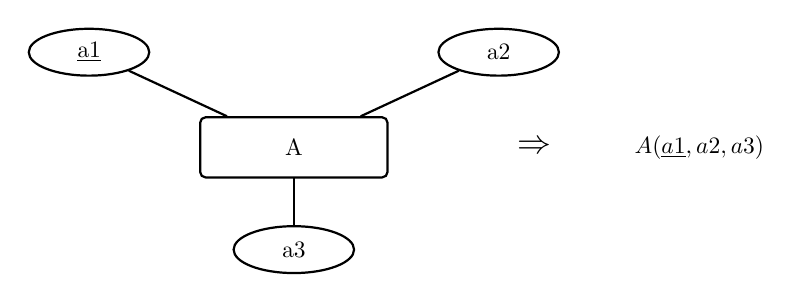
\begin{tikzpicture}[node distance=7mm and 10mm, scale=0.85, transform shape]
  \node[er/entity] (A) {A};
  \node[er/attribute, above left=of A] (a1) {\keyattr{a1}};
  \node[er/attribute, above right=of A] (a2) {a2};
  \node[er/attribute, below=of A] (a3) {a3};
  \draw[er/line] (A)--(a1);
  \draw[er/line] (A)--(a2);
  \draw[er/line] (A)--(a3);

  \node[right=18mm of A, font=\Large] (arrow) {$\Rightarrow$};
  \node[right=10mm of arrow, align=left] (rel) {$A(\keyattr{a1}, a2, a3)$};
\end{tikzpicture}
\end{frame}

% -----------------------------
\begin{frame}{Rules: Relationships with different Cardinality Constraints}
\begin{itemize}
  \item Relationship (with cardinality constraints). How many times min..max can/must an entity participate in the relationship set? 
  \item Use \textbf{min} (0 or 1) and \textbf{max} (1 or N) near each side.
\end{itemize}

\centering


\begin{tikzpicture}[scale=0.7, transform shape,node distance=8mm and 18mm]
  \node[er/entity] (player) {STUDENT};
  \node[er/entity, right=42mm of player] (team) {COURSE};
  \node[er/relationship] (playsIn) at ($(player)!0.5!(team)$) {EnrolledIn};
   \node[er/attribute, left=of player] (sid) {\keyattr{StudId}};
    \node[er/attribute, right=of team] (cid) {\keyattr{CourseId}};
    
  \draw[er/line] (player) -- (playsIn);
  \draw[er/line] (team) -- (playsIn);
  \draw[er/line] (player) -- (sid);
  \draw[er/line] (team) -- (cid);

  \node[er/card] at ($(team)!0.55!(playsIn)$) {0..M};
  \node[er/card] at ($(player)!0.55!(playsIn)$) {0..N};
\end{tikzpicture}
\small STUDENT(\underline{StudID}, ...),COURSE(\underline{CourseID}, ...), EnrolledIn(\underline{StudID}, \underline{CourseID}),\\
FK: EnrolledIn.StudId $\rightarrow$ STUDENT.StudId, EnrolledIn.CourseId $\rightarrow$ STUDENT.CourseId  


\begin{tikzpicture}[scale=0.7, transform shape,node distance=8mm and 18mm]
  \node[er/entity] (person) {PERSON};
  \node[er/entity, right=42mm of person] (car) {CAR};
  \node[er/relationship] (owns) at ($(person)!0.5!(car)$) {Owns};

  \draw[er/line] (person) -- (owns);
  \draw[er/line] (car) -- (owns);

  \node[er/card] at ($(person)!0.55!(owns)$) {0..N};
  \node[er/card] at ($(car)!0.55!(owns)$) {1..1};
  \node[er/attribute, left=of person] (sid2) {\keyattr{PersonId}};
  \node[er/attribute, right=of car] (cid2) {\keyattr{CarId}};
  \draw[er/line] (person) -- (sid2);
  \draw[er/line] (car) -- (cid2);
\end{tikzpicture}\\
\small PERSON(\underline{PersonId}, ...), CAR(\underline{CarID}, PersonId, ...), FK: CAR.PersonId $\rightarrow$ PERSON.PersonId \\
\textbf{Notably only two relations are used.}
\medskip

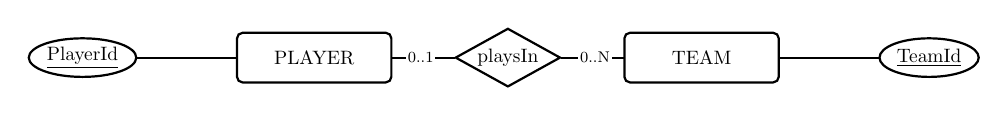
\begin{tikzpicture}[scale=0.7, transform shape,node distance=8mm and 18mm]
  \node[er/entity] (player2) {PLAYER};
  \node[er/entity, right=42mm of player2] (team2) {TEAM};
  \node[er/relationship] (playsIn2) at ($(player2)!0.5!(team2)$) {playsIn};
  \draw[er/line] (player2) -- (playsIn2);
  \draw[er/line] (team2) -- (playsIn2);

  \node[er/card] at ($(team2)!0.55!(playsIn2)$) {0..N};
  \node[er/card] at ($(player2)!0.55!(playsIn2)$) {0..1};
  \node[er/attribute, left=of player2] (sid3) {\keyattr{PlayerId}};
  \node[er/attribute, right=of team2] (cid3) {\keyattr{TeamId}};
  \draw[er/line] (player2) -- (sid3);
  \draw[er/line] (team2) -- (cid3);
\end{tikzpicture}\\

\small PLAYER(\underline{PlayerId},...), TEAM(\underline{TeamId},...), playsIn(\underline{PlayerId},..., TeamId),\\ FK: PlaysIn.PlayerId $\rightarrow$ PLAYER.PlayerId

\end{frame}

% -----------------------------
\begin{frame}{Rule: Weak Entity Set}
\begin{itemize}
  \item Recap: A \textbf{weak entity} cannot be uniquely identified by its own attributes alone.
  \item It is identified through an \textbf{identifying relationship} with a strong entity.
  \item Rule of thumb: max cardinality of weak entity in identifying relationship is often 1.
\end{itemize}

\centering
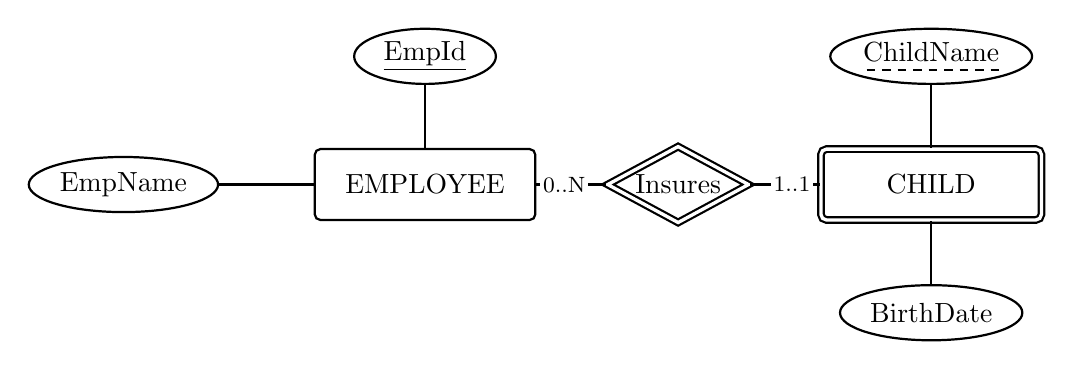
\begin{tikzpicture}[node distance=8mm and 12mm]
  \node[er/entity] (company) {EMPLOYEE};
  \node[er/weakentity, right=36mm of company] (dept) {CHILD};

  \node[er/identrel] (owns) at ($(company)!0.5!(dept)$) {Insures};

  \node[er/attribute, above=of company] (cid) {\keyattr{EmpId}};
  \node[er/attribute, left=of company] (ename) {EmpName};

  \node[er/attribute, above=of dept] (did) {\dashuline{ChildName}};
  \node[er/attribute, below=of dept] (dname) {BirthDate};

  \draw[er/line] (company) -- (owns);
  \draw[er/line] (dept) -- (owns);
  \draw[er/line] (company) -- (ename);

  \draw[er/line] (company) -- (cid);
  \draw[er/line] (dept) -- (did);
  \draw[er/line] (dept) -- (dname);

  \node[er/card] at ($(company)!0.55!(owns)$) {0..N};
  \node[er/card] at ($(dept)!0.55!(owns)$) {1..1};
\end{tikzpicture}

% --- FIX: removed undefined textblock environment; also put arrow in math mode
\vspace{1mm}
\begin{block}{Relational schema}
\footnotesize
\texttt{EMPLOYEE(\underline{EmpId}, EmpName)}\\
\texttt{CHILD(\underline{EmpId}, \underline{ChildName}, BirthDate)}\\
$\texttt{CHILD.EmpId} \rightarrow \texttt{EMPLOYEE.EmpId}$
\end{block}

\end{frame}

% -----------------------------
\begin{frame}{Rule: Transforming Attributes}
\small
\begin{itemize}
  \item \textbf{Rule (Derived attributes)}: discard derived attributes (compute when needed).
  \item \textbf{Rule (Composite attributes)}: replace a composite attribute by its components; discard the composite node.
  \item \textbf{Rule (Multivalued attributes)}: create a separate ``attribute relation'' containing:
  \begin{itemize}
    \item the key of the owner entity set, and
    \item the multivalued attribute
  \end{itemize}
  and make the owner key a foreign key.
\end{itemize}

\vspace{2mm}
\centering
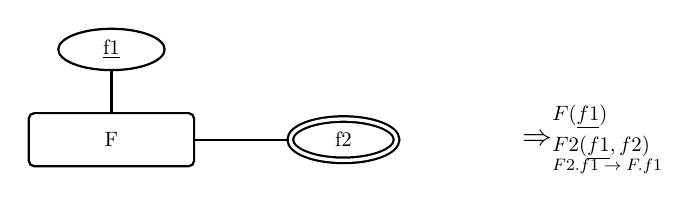
\begin{tikzpicture}[node distance=7mm and 10mm, scale=0.75, transform shape]
  \node[er/entity] (F) {F};
  \node[er/attribute, above=of F] (f1) {\keyattr{f1}};
  \node[er/multival, right=16mm of F] (f2) {f2};
  \draw[er/line] (F)--(f1);
  \draw[er/line] (F)--(f2);
  \node[right=20mm of f2, font=\Large] {$\Rightarrow$};
  \node[right=10mm of f2, xshift=15mm, align=left] {$F(\keyattr{f1})$\\[1mm]$F2(\keyattr{f1}, f2)$\\[-1mm]\footnotesize $F2.f1 \rightarrow F.f1$};
\end{tikzpicture}
\end{frame}

% -----------------------------
\begin{frame}{Note on Cardinalities (in these rules)}
\small
\begin{itemize}
  \item In the transformation rules below, cardinalities refer to \textbf{maximum} cardinalities.
  \item A 0:1 relationship means max participation of an entity in a relationship is 1 (e.g., ``a person can be in at most one active marriage'').
    \item A 1:1 relationship means exact cardinality is 1 (e.g., ``a car has exactly one registration'').
  \item In the relational model, \textbf{minimum} cardinality is generally not expressible in the standard ER model;
        additional integrity constraints are needed (we can encode them later, e.g., in SQL).
\end{itemize}
\end{frame}

% -----------------------------
\begin{frame}{Recap: Abstraction Structures (EER)}
\begin{columns}[T,onlytextwidth]
\column{0.48\textwidth}
\begin{itemize}
  \item Use \textbf{E}xtended ER (EER) to model inheritance-like structures.
  \item A \textbf{super-entity} has shared attributes.
  \item \textbf{sub-entities} specialize it (e.g., STUDENT, STAFF).
  \item Subtypes can have specific relationships (e.g. STAFF has CONTRACT)
  \item Disjoint vs overlapping; total vs partial.
  \begin{itemize}
  \item Supertype: \textbf{PERSON}; subtypes: \textbf{STUDENT}, \textbf{STAFF} (U-marks = children; 1/2 lines = partial/total coverage).
  \item Circle label: \textbf{d} = disjoint, \textbf{o} = overlapping.
\end{itemize}
\end{itemize}

\column{0.52\textwidth}
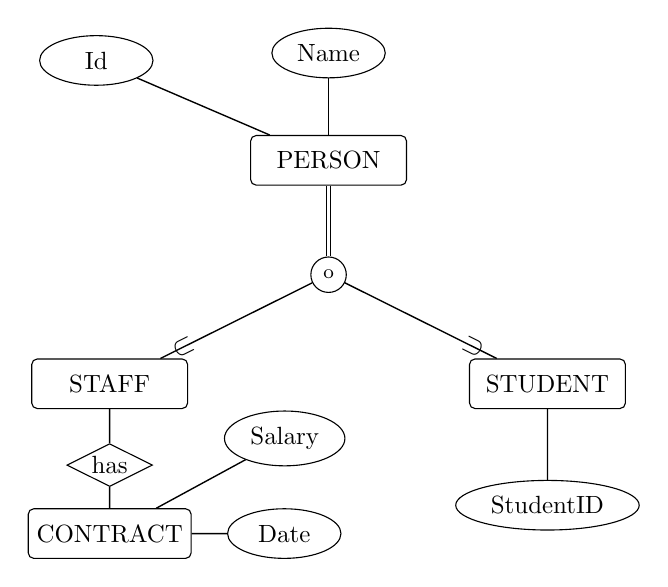
\begin{tikzpicture}[
  scale=0.9, transform shape,
  node distance=8mm and 16mm,
  entity/.style={draw, rectangle, rounded corners=2pt, minimum width=22mm, minimum height=7mm, align=center},
  attr/.style={draw, ellipse, minimum width=16mm, minimum height=7mm, align=center},
  rel/.style={draw, diamond, aspect=2, inner sep=1pt, align=center},
  line/.style={draw, line width=0.5pt},
  isa/.style={draw, circle, inner sep=0pt, minimum size=5mm, font=\footnotesize}
]

\node[entity] (person) {PERSON};
\node[attr, above left=of person] (pid) {Id};
\node[attr, above=of person] (name) {Name};
\draw[line] (person) -- (pid);
\draw[line] (person) -- (name);

\node[isa, below=10mm of person] (isa) {o};

\node[entity, below left=10mm and 18mm of isa] (staff) {STAFF};
\node[entity, below right=10mm and 18mm of isa] (stud) {STUDENT};

\draw[line, double, double distance=0.8pt] (person) -- (isa);

\draw[line,
  postaction={decorate},
  decoration={markings,
    mark=at position 0.85 with {
      \node[sloped,allow upside down,inner sep=0pt,rotate=90] {$\cup$};
    }
  }
] (isa) -- (staff);

\draw[line,
  postaction={decorate},
  decoration={markings,
    mark=at position 0.85 with {
      \node[sloped,allow upside down,inner sep=0pt,rotate=90] {$\cup$};
    }
  }
] (isa) -- (stud);

\node[attr, below=10mm of stud] (sid) {StudentID};
\draw[line] (stud) -- (sid);

\node[entity, below=14mm of staff] (contract) {CONTRACT};
\node[attr, above right=10mm of contract] (salary) {Salary};
\node[attr, right=5mm of contract] (cdate) {Date};
\draw[line] (contract) -- (salary);
\draw[line] (contract) -- (cdate);

\node[rel, above=3mm of contract] (has) {has};
\draw[line] (staff) -- (has);
\draw[line] (has) -- (contract);

\end{tikzpicture}

\end{columns}
\end{frame}

% -----------------------------
\begin{frame}{Transforming Abstraction Structures (EER)}
\small
There are (at least) four common approaches:
\begin{enumerate}
  \item \textbf{Way 1}: one relation for each super- and sub-entity set; sub-relation key includes super key.
  \item \textbf{Way 2}: one relation for each sub-entity set; include both sub and super attributes.
  \item \textbf{Way 3}: one relation for the whole hierarchy; add one \texttt{type} attribute (may lead to many NULLs).
  \item \textbf{Way 4}: like Way 3, but use boolean ``flags'' (e.g., \texttt{isStaff}, \texttt{isStudent}).
\end{enumerate}
\begin{figure}
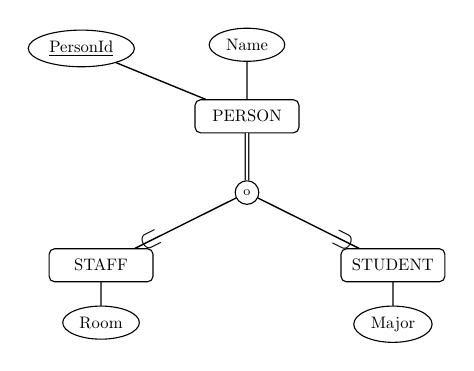
\begin{tikzpicture}[
  scale=0.6, transform shape,
  node distance=8mm and 16mm,
  entity/.style={draw, rectangle, rounded corners=2pt, minimum width=22mm, minimum height=7mm, align=center},
  attr/.style={draw, ellipse, minimum width=16mm, minimum height=7mm, align=center},
  rel/.style={draw, diamond, aspect=2, inner sep=1pt, align=center},
  line/.style={draw, line width=0.5pt},
  isa/.style={draw, circle, inner sep=0pt, minimum size=5mm, font=\footnotesize}
]

\node[entity] (person) {PERSON};
\node[attr, above left=of person] (pid) {\underline{PersonId}};
\node[attr, above=of person] (name) {Name};
\draw[line] (person) -- (pid);
\draw[line] (person) -- (name);

\node[isa, below=10mm of person] (isa) {o};

\node[entity, below left=10mm and 18mm of isa] (staff) {STAFF};
\node[entity, below right=10mm and 18mm of isa] (stud) {STUDENT};

\draw[line, double, double distance=0.8pt] (person) -- (isa);

\draw[line,
  postaction={decorate},
  decoration={markings,
    mark=at position 0.85 with {
      \node[sloped,allow upside down,inner sep=0pt,rotate=90] {$\cup$};
    }
  }
] (isa) -- (staff);

\draw[line,
  postaction={decorate},
  decoration={markings,
    mark=at position 0.85 with {
      \node[sloped,allow upside down,inner sep=0pt,rotate=90] {$\cup$};
    }
  }
] (isa) -- (stud);

\node[attr, below=5mm of stud] (sid) {Major};
\draw[line] (stud) -- (sid);

\node[attr, below=5mm of staff] (room) {Room};
\draw[line] (staff) -- (room);

\end{tikzpicture}$\quad$
\begin{minipage}{0.4\linewidth}
\vspace{-3.5cm}

{\small
\textbf{Way 1:}\\ PERSON(\underline{PersonId},Name)\\
STAFF(\underline{PersonId}, room)\\
STUDENT(\underline{PersonId},Major)\\
FK: STAFF.PersonId$\rightarrow$PERSON.PersonId,\\
STUDENT.PersonId$\rightarrow$PERSON.PersonId

\textbf{Way 3:}\\ PERSON(\underline{PersonId},Name, Room, Major, \\
IsStaff:bool, IsStudent:bool)}
\end{minipage}
\end{figure}
\end{frame}

% -----------------------------
\begin{frame}{Heuristics for Abstraction Structures (translated labels)}
\vspace{1mm}
\begin{itemize}
  \item \textbf{Disjoint + Total}: often choose Way 2 (or Way 3 if acceptable NULLs).
  \item \textbf{Disjoint + Partial}: often choose Way 1 (avoid repetition).
  \item \textbf{Overlapping + Total}: often choose Way 4 (flags), otherwise Way 1.
  \item \textbf{Overlapping + Partial}: often choose Way 4; otherwise, Way 1 (be careful with repetition).
\end{itemize}
\textbf{Key Decision Principle:} Use keys to enforce constraints and avoid redundancy.
\end{frame}

% -----------------------------
\begin{frame}{Applying Rules (practical advice)}
\small
\begin{itemize}
  \item Real ER diagrams may trigger multiple rules; there are exceptions.
  \item A general approach:
  \begin{enumerate}
    \item transform entity sets,
    \item transform attributes,
    \item transform relationship sets,
    \item transform abstraction structures.
  \end{enumerate}
  \item If several rules could apply:
  \begin{itemize}
    \item try suitable rules sequentially,
    \item compare results from the database viewpoint (fewer relations, clearer structure, fewer NULLs).
  \end{itemize}
  \item All relationships (except identifying ones) can always be transformed via Rule 8 by creating a relationship relation
        (but you may need to normalize later).
  \item Way 1 for abstraction structures always works, but can cause repetition.
\end{itemize}
\end{frame}

% -----------------------------
\begin{frame}{Summary}
\small
\begin{itemize}
  \item The relational model represents data as relations (tables) with strict structural properties.
  \item Keys: candidate keys and primary keys ensure identifiability; foreign keys represent references and enforce integrity.
  \item Transformation rules provide a systematic mapping from ER/EER designs to relational schemas.
  \item When multiple transformations are possible, choose the one that fits the domain and leads to a clean schema.
\end{itemize}
\end{frame}

\end{document}
